% !TeX program = xelatex
\documentclass[UTF8,aspectratio=169,10pt]{ctexbeamer}
\usepackage{amsmath,amssymb,booktabs,graphicx}
\usetheme{default}
\definecolor{ink}{RGB}{35,59,79}
\setbeamercolor{structure}{fg=ink}
\setbeamercolor{frametitle}{fg=ink}
\setbeamercolor{normal text}{fg=black,bg=white}
\setbeamertemplate{navigation symbols}{}
\setbeamertemplate{footline}{\hfill\usebeamerfont{page number in head/foot}\insertframenumber\,/\,\inserttotalframenumber\hspace{5mm}\vspace{3mm}}
\setbeamersize{text margin left=9mm,text margin right=9mm}
\setbeamerfont{frametitle}{size=\Large}
\setbeamertemplate{itemize items}[circle]
\setlength{\parskip}{5pt}
\graphicspath{{images/}}
\newcommand{\source}[1]{\vfill{\tiny\color{gray}资料：#1\par}}
\title{多任务学习：阅读与初步实验}
\subtitle{Uncertainty Weighting、GradNorm}
\author{廖望}
\date{2026年11月}
\begin{document}

\begin{frame}
\titlepage
\end{frame}

\begin{frame}{多任务学习与任务权重}
针对同一个输入，需要输出两个甚至更多预测结果，多个预测结果之间如何进行 trade-off 是一个重要问题。
\medskip
\begin{itemize}\setlength{\itemsep}{9pt}
\item 网络参数分为共享参数 $\theta_s$ 与任务 $i$ 专属参数 $\theta_i$。
\item 任务 $i$ 的损失表示为 $L_i(\theta_s,\theta_i)$。
\item 通常优化加权目标，其中 $w_i$ 是相应任务的权重：
\[\mathcal J=\sum_i w_iL_i(\theta_s,\theta_i).\]
\end{itemize}
\medskip
预先固定 $w_i$ 是一种方向。既然损失通过梯度下降来优化，是否存在一种合理的方法，使得我们可以动态地、对结果有利地更新 $w_i$？
\end{frame}

\begin{frame}{Uncertainty Weighting：回归任务}

设模型对 $x$ 的回归预测为 $f(x;\theta)$，令观测服从高斯分布：
\[p(y\mid x,\theta,\sigma)=\mathcal N\!\left(y;f(x;\theta),\sigma^2\right).\]
对应的负对数似然为
\[
-\log p(y\mid x,\theta,\sigma)
=\frac{1}{2\sigma^2}\left(y-f(x;\theta)\right)^2+\log\sigma+C.
\]
将平方误差记为 $\mathcal L_{\rm reg}$，可写作
\[
\mathcal J_{\rm reg}(\theta,\sigma)
=\frac{1}{2\sigma^2}\mathcal L_{\rm reg}(\theta)+\log\sigma.
\]
\medskip
多个回归任务假设独立的情况下，联合概率取对数后相加，即可得到多任务目标。
\end{frame}

\begin{frame}{Uncertainty Weighting：分类任务}
对分类任务，引入如下 Softmax：
\[
p(y=c\mid\boldsymbol z,\sigma)
=\frac{\exp(z_c/\sigma^2)}{\sum_k\exp(z_k/\sigma^2)}.
\]
取负对数后可得
\[
-\log p(y=c\mid\boldsymbol z,\sigma)
=\frac{1}{\sigma^2}\mathcal L_{\rm CE}(\boldsymbol z,c)
+R(\boldsymbol z,\sigma).
\]
利用论文中的近似
\[
\frac1\sigma\sum_k\exp(z_k/\sigma^2)
\approx\left(\sum_k\exp z_k\right)^{1/\sigma^2},
\]
可近似得到
\[
\mathcal J_{\rm cls}\approx\frac1{\sigma^2}\mathcal L_{\rm CE}+\log\sigma.
\]
将回归与分类任务的 $\mathcal J$ 相加，得到最终优化目标。实际学习 $s=\log\sigma^2$ 比较方便。
\end{frame}

\begin{frame}{Uncertainty Weighting：论文中的实验结果}
Kendall et al. (2018) 在 Tiny Cityscapes 上训练三个任务：语义分割、实例分割与深度估计。
\begin{center}
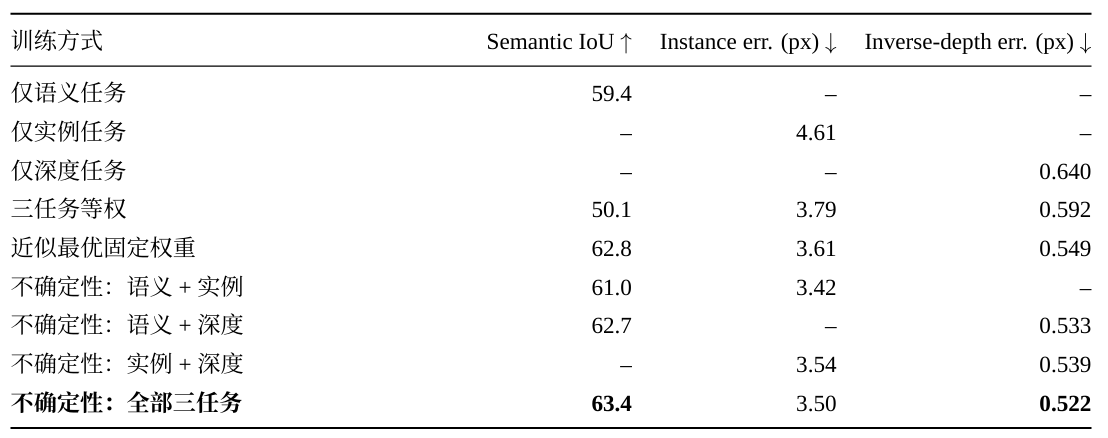
\includegraphics[width=0.96\linewidth,height=0.58\textheight,keepaspectratio]{table_1.png}
\end{center}
\small 笔记中记录的结果：Uncertainty 三任务训练的 Semantic IoU 为 63.4，实例误差为 3.50，逆深度误差为 0.522，整体表现良好。
\end{frame}

\begin{frame}{GradNorm：梯度范数与相对训练速度}

考虑多任务训练步 $t$，选取一组共享网络参数 $\mathcal W$，取加权梯度向量的范数：
\[
G_i(t)=\left\|\nabla_{\mathcal W}[w_i(t)L_i(t)]\right\|_2.
\]
首先计算所有 $G_i$ 的平均值 $\bar G$，并计算相对初始损失：
\[
\bar G(t)=\frac1T\sum_{i=1}^{T}G_i(t),\qquad
\widetilde L_i(t)=\frac{L_i(t)}{L_i(0)}.
\]
再定义
\[
r_i(t)=\frac{T\widetilde L_i(t)}{\sum_j\widetilde L_j(t)}.
\]
\end{frame}

\begin{frame}{GradNorm：目标梯度与辅助损失}
令目标梯度范数为
\[
G_i^{\rm target}(t)=\bar G(t)[r_i(t)]^\alpha,
\]
其中 $\alpha$ 是超参数。
\medskip

定义梯度平衡辅助损失：
\[
\mathcal L_{\rm grad}(t;w)
=\sum_{i=1}^{T}\left|G_i(t)
-\operatorname{stopgrad}\!\left(G_i^{\rm target}(t)\right)\right|.
\]
\medskip
根据该辅助损失调整任务权重 $w$，使加权梯度范数接近相应目标。
\end{frame}

\begin{frame}{GradNorm：论文中的实验结果}
\begin{center}
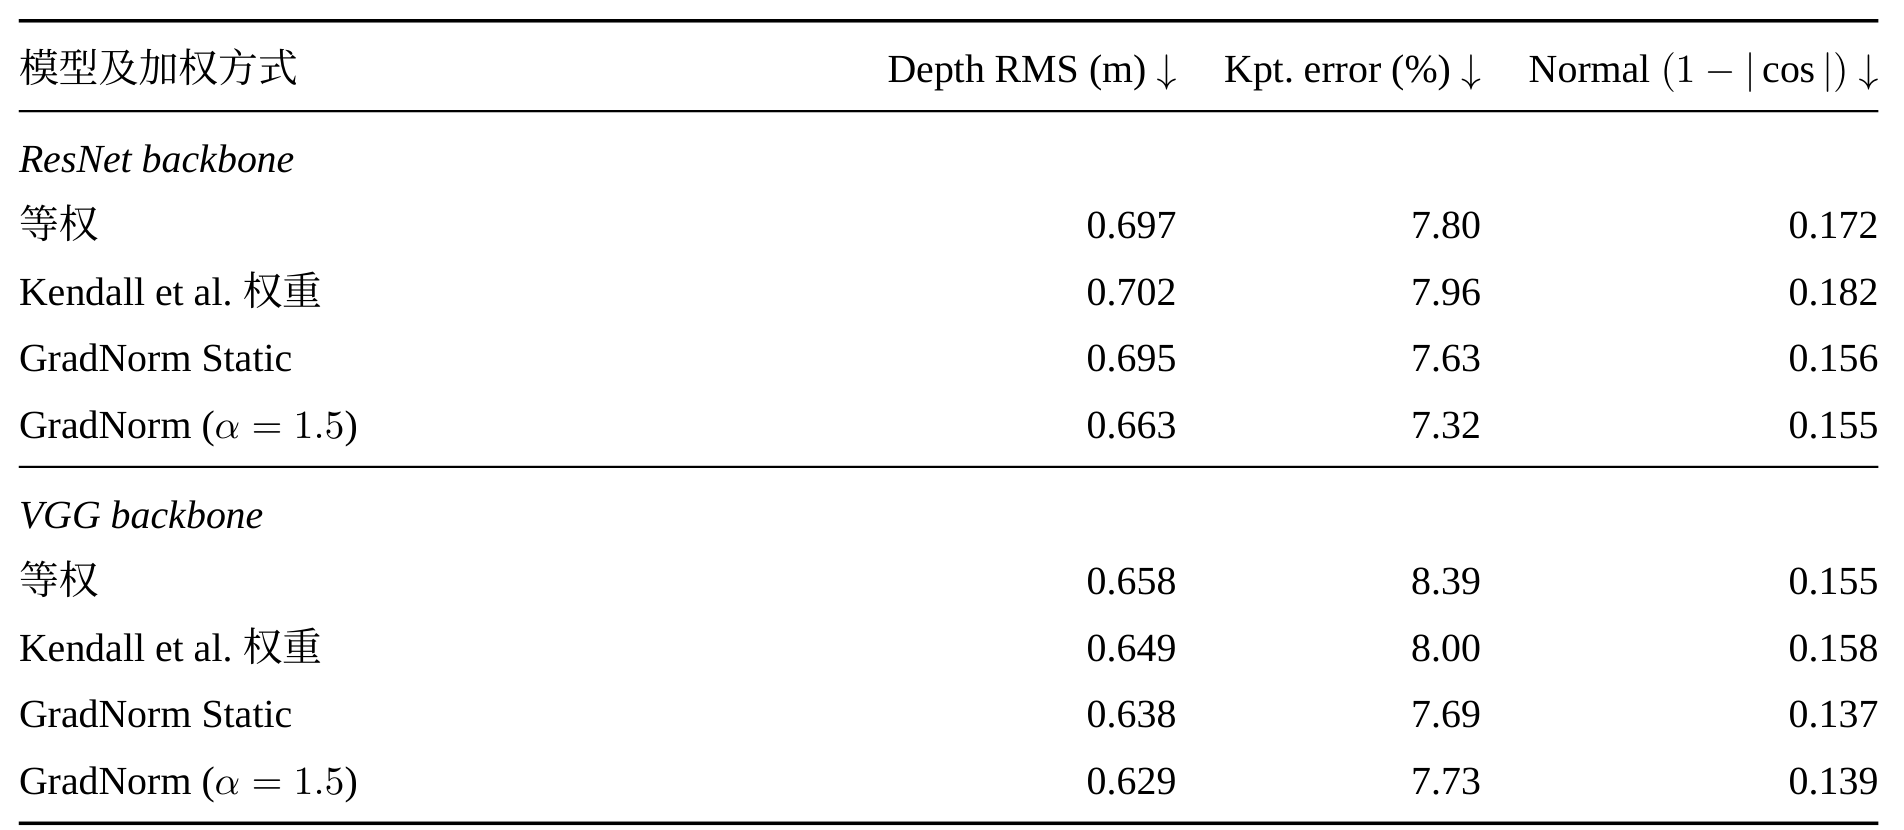
\includegraphics[width=0.94\linewidth,height=0.70\textheight,keepaspectratio]{table_2.png}
\end{center}
\end{frame}

\begin{frame}{实验经过与 GPT 的参与}
\begin{enumerate}\setlength{\itemsep}{10pt}
\item \textbf{我的初始想法：}在 CIFAR-100 上，用 Fine（100 细类）与 Coarse（20 粗类）比较 GradNorm、Uncertainty 和等权训练。
\item \textbf{我的后续想法：}加入噪声，观察调权方法的变化。已完成标签噪声、训练特征高斯噪声等对照。
\item \textbf{遇到的问题：}Fine 与 Coarse 任务很接近，Coarse 由 Fine 唯一确定。前期实验中，动态加权的平均收益很小。
\item \textbf{GPT 协助扩展：}我让 GPT 构思并完成新的异质任务实验，包括 Fine + Color、Fine + Rotation，并在 GPT 指导下引入 PCGrad。
\end{enumerate}
\end{frame}

\begin{frame}{Fine + Coarse}
\begin{columns}[T,onlytextwidth]
\begin{column}{0.49\textwidth}
\centering
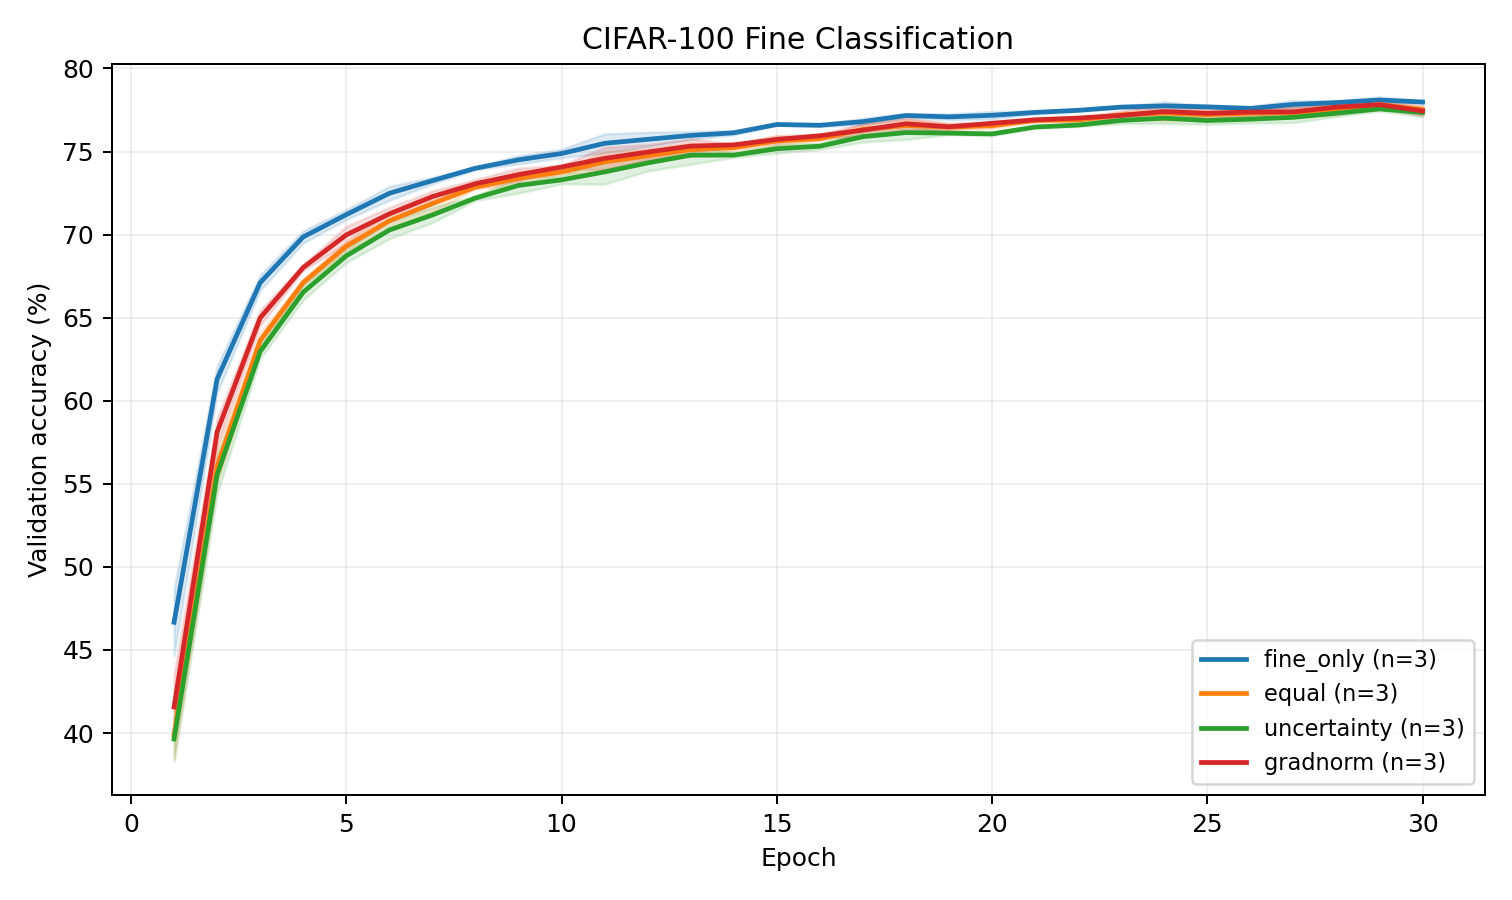
\includegraphics[width=\linewidth]{clean_validation_fine.png}
\par\small Fine 验证准确率
\end{column}
\begin{column}{0.49\textwidth}
\centering
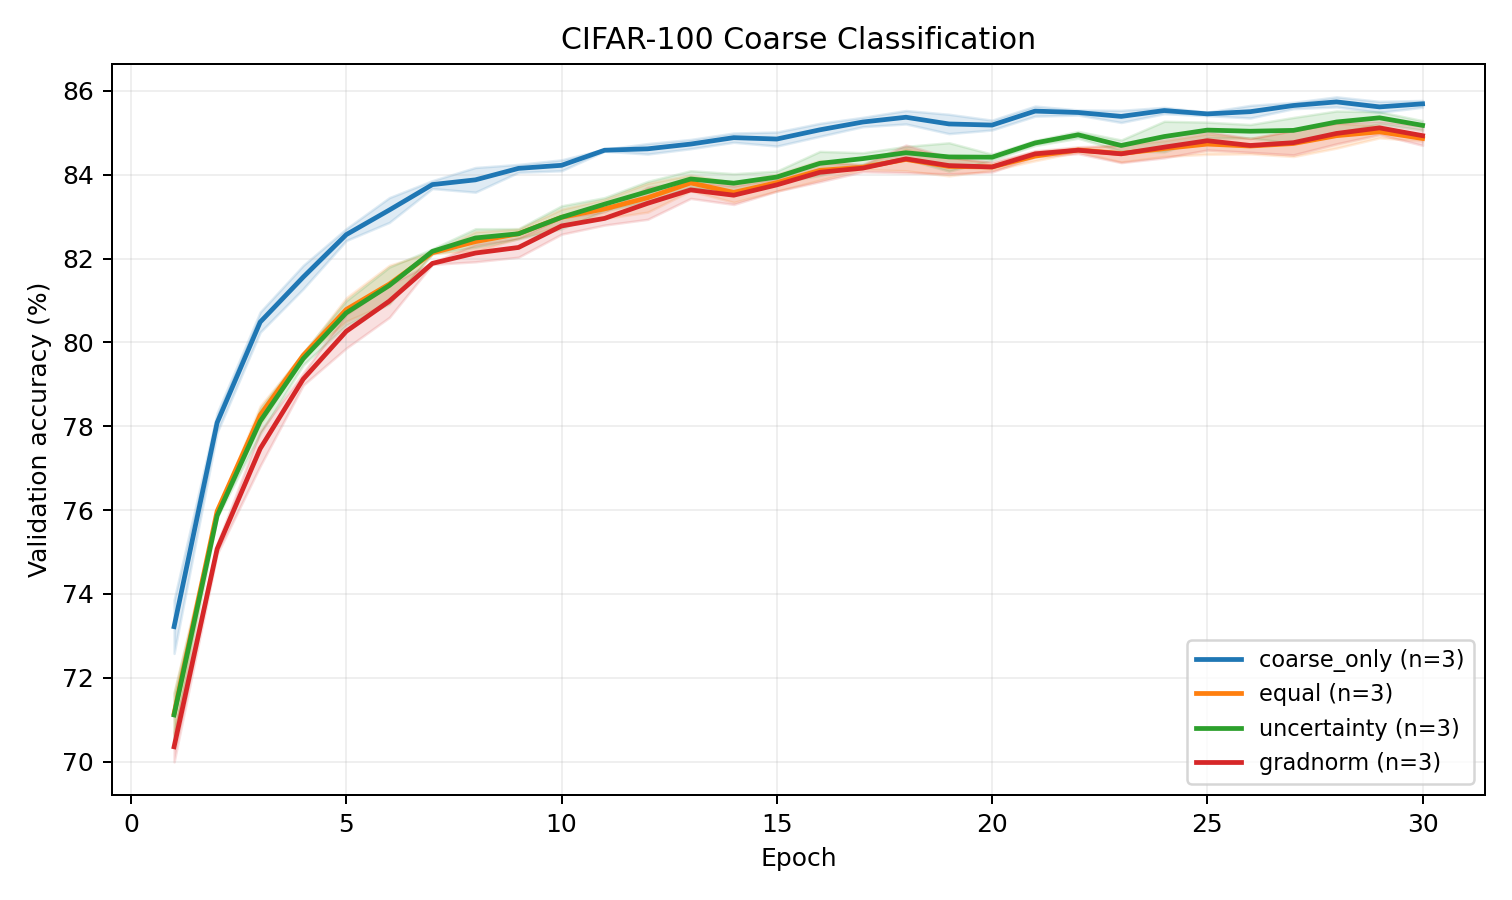
\includegraphics[width=\linewidth]{clean_validation_coarse.png}
\par\small Coarse 验证准确率
\end{column}
\end{columns}
\medskip
\begin{itemize}\setlength{\itemsep}{5pt}
\item Equal、Uncertainty、GradNorm 的曲线较接近，训练后期没有明显拉开差距，单任务曲线整体略高。
\item 对应测试集上，两任务平均准确率相对 Equal 仅提高约 0.06、0.09 pp。
\end{itemize}
\end{frame}

\begin{frame}{Fine + Coarse：加入标签噪声}
\begin{columns}[T,onlytextwidth]
\begin{column}{0.49\textwidth}
\centering
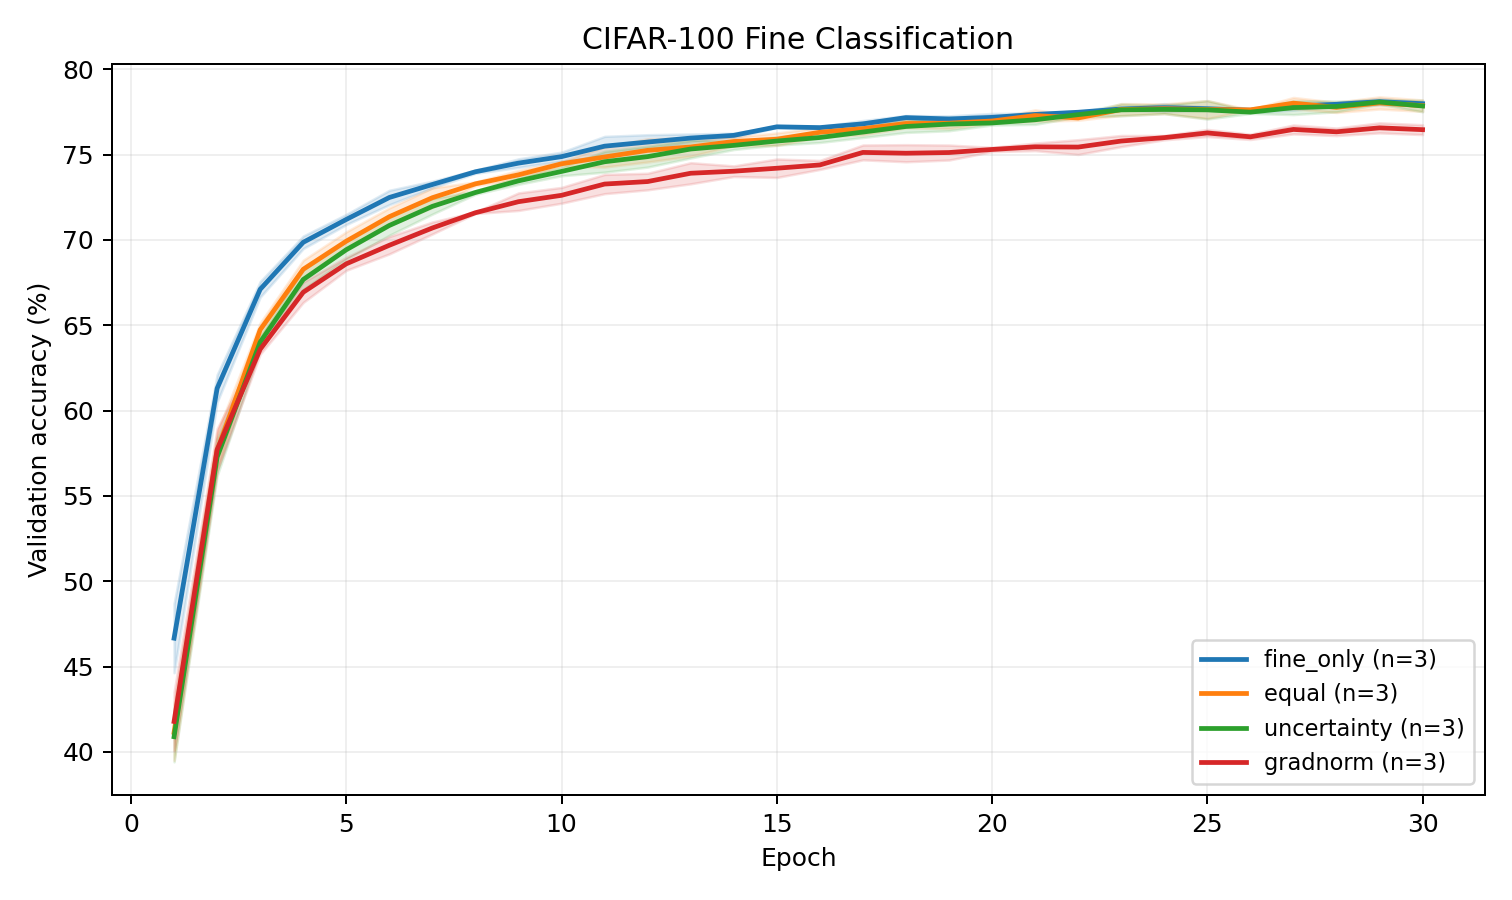
\includegraphics[width=\linewidth]{coarse20_validation_fine.png}
\par\small Fine 验证准确率
\end{column}
\begin{column}{0.49\textwidth}
\centering
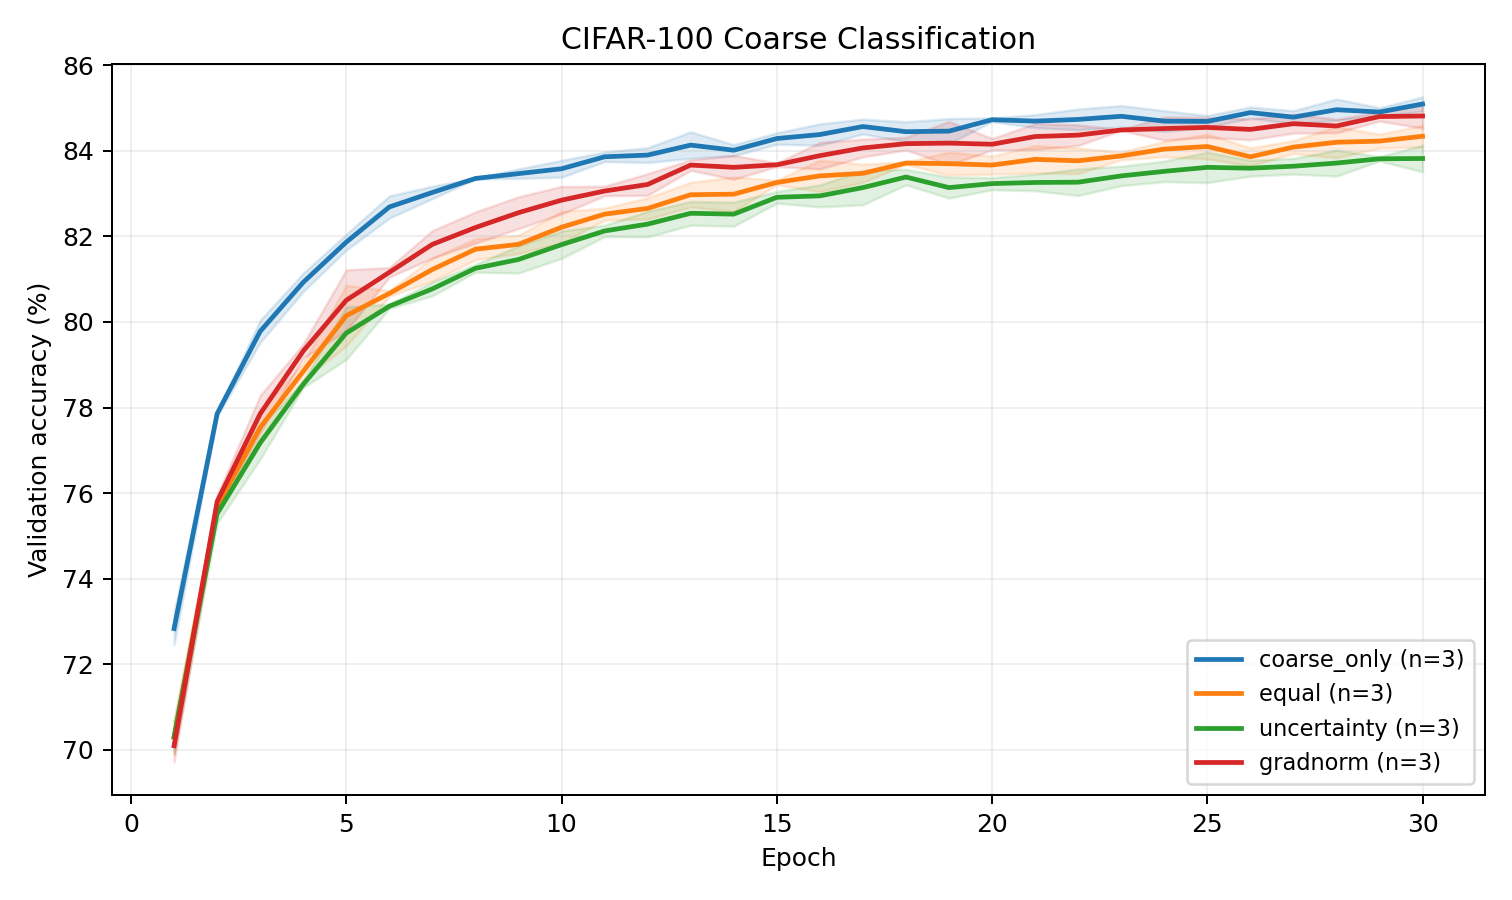
\includegraphics[width=\linewidth]{coarse20_validation_coarse.png}
\par\small Coarse 验证准确率
\end{column}
\end{columns}
\medskip

\begin{itemize}\setlength{\itemsep}{5pt}
\item 仅将训练集 Coarse 标签以 20\% 概率翻转到其他类别。
\item GradNorm 的 Coarse 曲线高于 Equal，但 Fine 曲线明显更低，变化主要体现为两项任务之间的取舍。
\end{itemize}
\end{frame}

\begin{frame}{后续实验：Fine + Rotation 的设置}
\begin{itemize}\setlength{\itemsep}{7pt}
\item \textbf{任务：}100 类物体识别与四类旋转预测（$0^\circ,90^\circ,180^\circ,270^\circ$）。两个任务使用同一旋转图像的特征。
\item \textbf{模型：}冻结本地 OpenCLIP ViT-B/32 图像编码器，训练共享 MLP（$512\to256\to256$）及两个任务头。
\item \textbf{数据：}45,000 训练、5,000 验证、10,000 测试，划分固定。先旋转图像，再提取特征。
\item \textbf{比较：}两个单任务参照、Equal、Uncertainty、GradNorm、PCGrad。每种方法 3 个种子、30 epochs。
\item \textbf{评价：}多任务按验证集两项准确率平均选模型，再报告测试结果。Fine 只评原图，Rotation 评四角度。
\end{itemize}
\end{frame}

\begin{frame}{Fine + Rotation}
\begin{center}
\begin{tabular}{lccc}
\toprule
方法 & Fine & Rotation & 两任务平均\\
\midrule
Fine-only & $73.07\pm0.42$ & --- & ---\\
Rotation-only & --- & $56.02\pm0.39$ & ---\\
Equal & $72.45\pm0.12$ & $55.20\pm0.04$ & $63.83\pm0.05$\\
Uncertainty & $71.80\pm0.35$ & $55.16\pm0.35$ & $63.48\pm0.33$\\
GradNorm & $71.16\pm0.18$ & $56.04\pm0.15$ & $63.60\pm0.16$\\
PCGrad & $72.57\pm0.25$ & $55.30\pm0.23$ & $63.93\pm0.24$\\
\bottomrule
\end{tabular}
\end{center}
\normalsize
\begin{itemize}\setlength{\itemsep}{6pt}
\item GradNorm 相对 Equal：Fine $-1.29$ pp，Rotation $+0.84$ pp，两项变化在三个种子上方向一致。
\item PCGrad 平均分约 $+0.11$ pp，三个种子中两次略降、一次提高。
\end{itemize}
\end{frame}

\begin{frame}{Fine + Rotation：两项任务的准确率曲线}
\begin{columns}[T,onlytextwidth]
\begin{column}{0.49\textwidth}
\centering
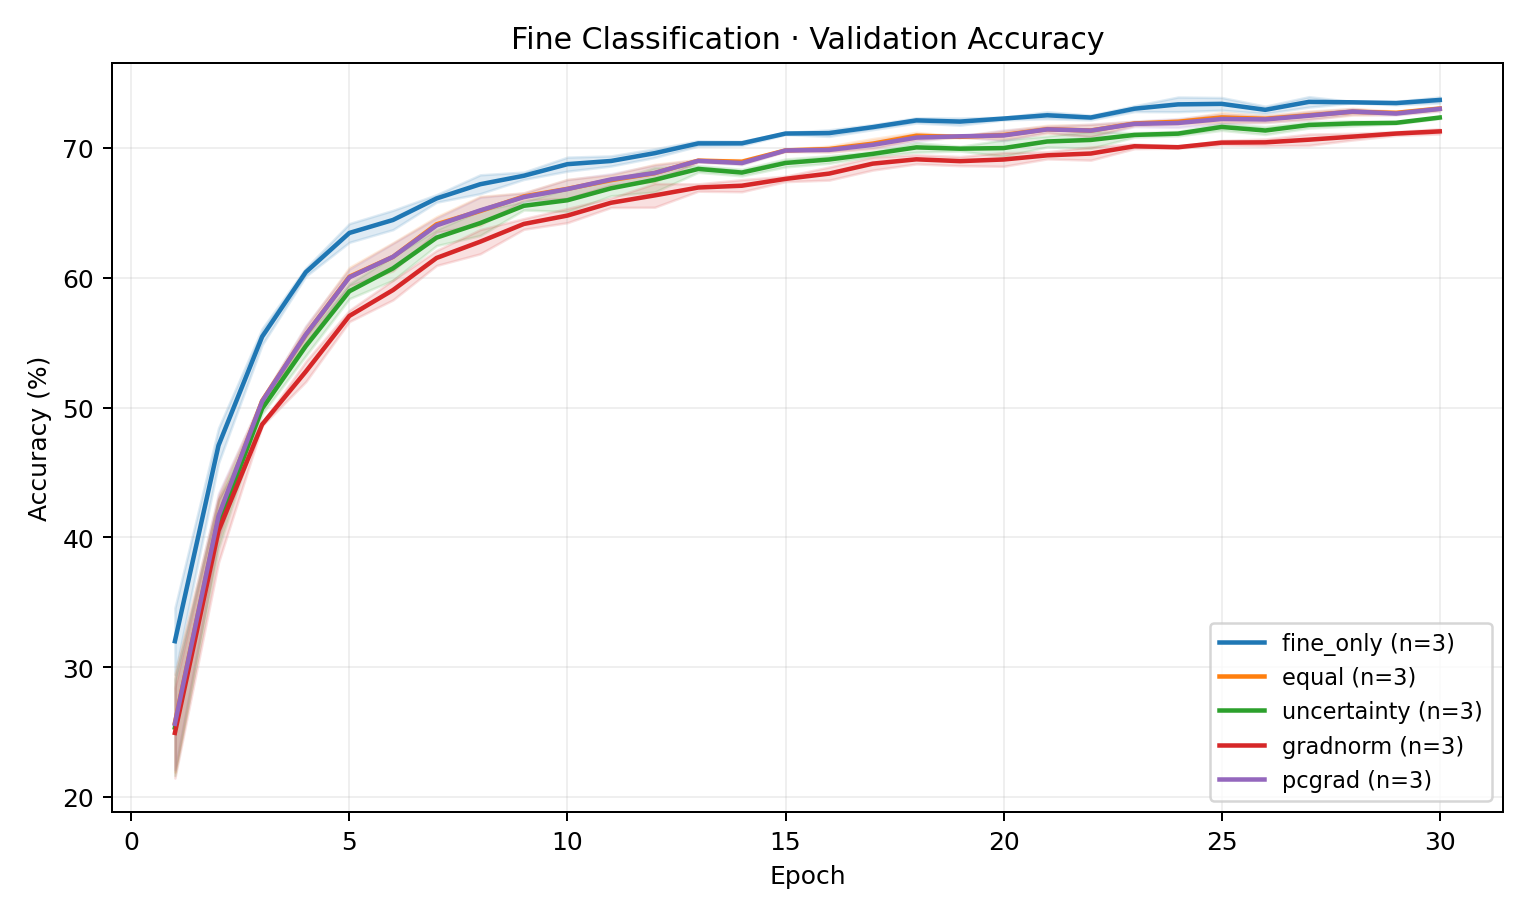
\includegraphics[width=\linewidth]{rotation_validation_fine.png}
\par\small Fine 验证准确率（仅 $0^\circ$）
\end{column}
\begin{column}{0.49\textwidth}
\centering
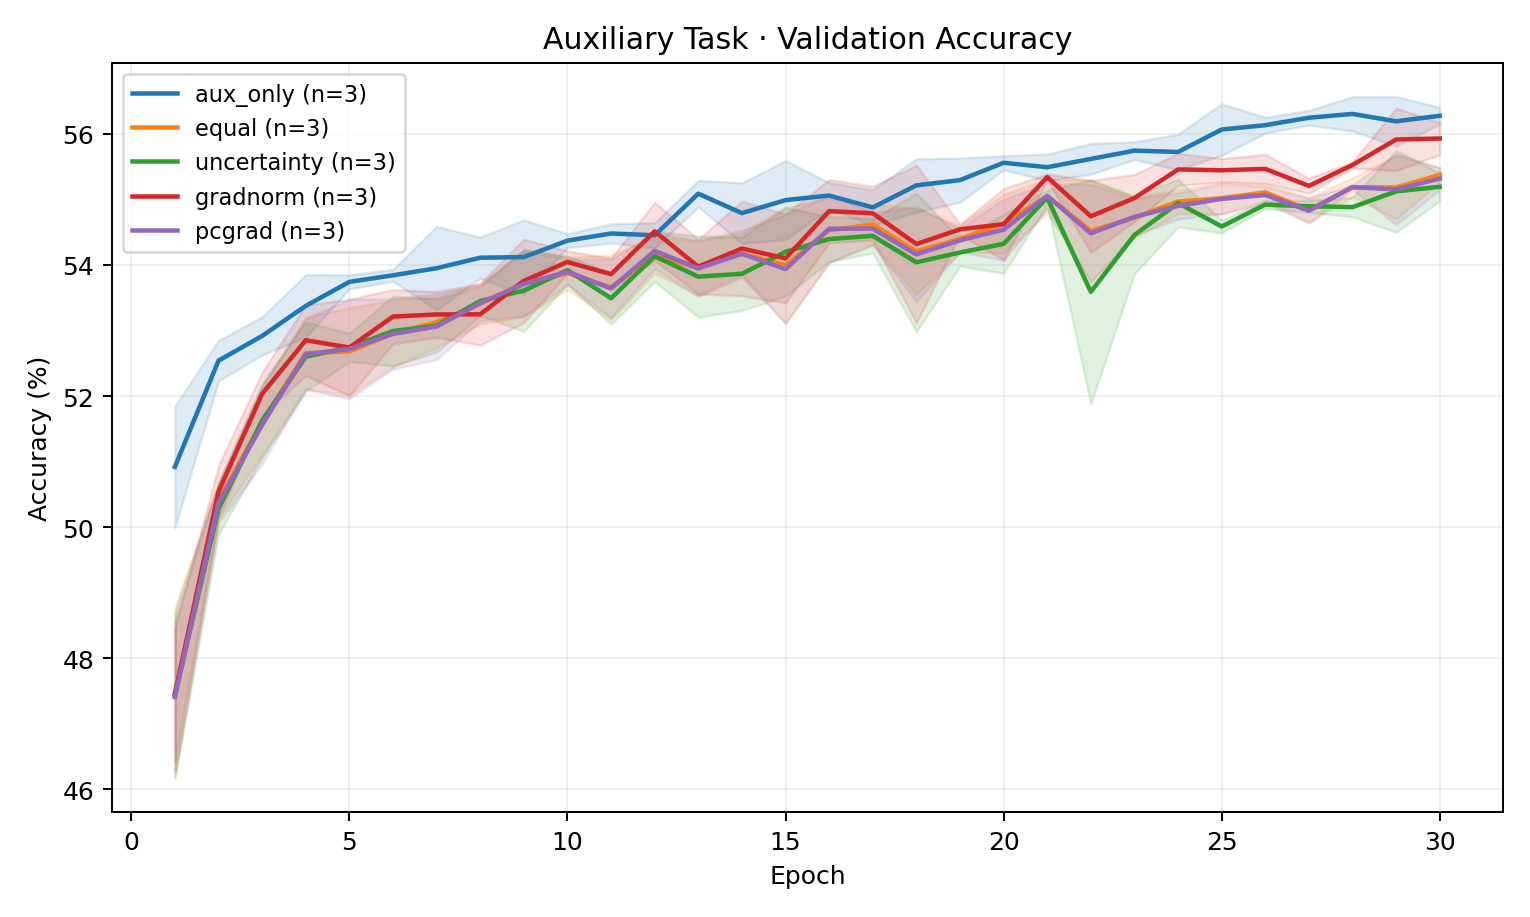
\includegraphics[width=\linewidth]{rotation_validation_aux.png}
\par\small Rotation 验证准确率（四角度）
\end{column}
\end{columns}
\medskip
\begin{itemize}\setlength{\itemsep}{5pt}
\item GradNorm 在 Fine 上整体偏低，在 Rotation 后期相对较高。
\item Equal 与 PCGrad 的验证曲线较接近。
\end{itemize}
\end{frame}

\begin{frame}{本次学习与实验记录}
\begin{itemize}\setlength{\itemsep}{5pt}
\item 阅读 Uncertainty Weighting 与 GradNorm，整理了概率推导、梯度平衡公式和论文中的实验结果。
\item 最初尝试 CIFAR-100 Fine + Coarse，随后加入噪声与少样本对照。
\item 让 GPT 构思并完成异质任务实验，并在 GPT 指导下加入 PCGrad。
\item 目前结果中，GradNorm 的变化主要体现在两项任务的取舍上，PCGrad 的平均提升较小。
\end{itemize}
\end{frame}
\end{document}
